\documentclass[8pt,aspectratio=169]{beamer}
\usetheme{Madrid}
\usepackage{graphicx,booktabs,adjustbox,multicol,amsmath,amssymb,listings,xcolor}
\definecolor{mlblue}{RGB}{0,102,204}
\definecolor{mlpurple}{RGB}{51,51,178}
\definecolor{mllavender}{RGB}{173,173,224}
\definecolor{mllavender2}{RGB}{193,193,232}
\definecolor{mllavender3}{RGB}{204,204,235}
\definecolor{mllavender4}{RGB}{214,214,239}
\definecolor{mlorange}{RGB}{255,127,14}
\definecolor{mlgreen}{RGB}{44,160,44}
\definecolor{mlred}{RGB}{214,39,40}
\definecolor{mlgray}{RGB}{127,127,127}
\setbeamercolor{palette primary}{bg=mllavender3,fg=mlpurple}
\setbeamercolor{palette secondary}{bg=mllavender2,fg=mlpurple}
\setbeamercolor{palette tertiary}{bg=mllavender,fg=white}
\setbeamercolor{palette quaternary}{bg=mlpurple,fg=white}
\setbeamercolor{structure}{fg=mlpurple}
\setbeamercolor{title}{fg=mlpurple}
\setbeamercolor{frametitle}{fg=mlpurple,bg=mllavender3}
\setbeamercolor{block title}{bg=mllavender2,fg=mlpurple}
\setbeamercolor{block body}{bg=mllavender4,fg=black}
\setbeamertemplate{navigation symbols}{}
\setbeamertemplate{itemize items}[circle]
\setbeamersize{text margin left=5mm,text margin right=5mm}
\newcommand{\bottomnote}[1]{\vfill\vspace{-2mm}\textcolor{mllavender2}{\rule{\textwidth}{0.4pt}}\vspace{1mm}\footnotesize\textbf{#1}}
\usepackage{tikz,pgfplots}
\pgfplotsset{compat=1.18}
\usetikzlibrary{arrows.meta,positioning,shapes.geometric,calc}
\title{Layer 2 Scaling Solutions: Course Preview}
\subtitle{INTRO Preview}
\author{Prof.~Dr.~Joerg Osterrieder}
\institute{University Lecture Series}
\date{\today}
\begin{document}

% Frame 1: Title
\begin{frame}
\titlepage
\end{frame}

% Frame 2: Why Layer 2 Scaling Matters
\begin{frame}{Why Layer 2 Scaling Matters}
\begin{columns}[T]
\begin{column}{0.62\textwidth}
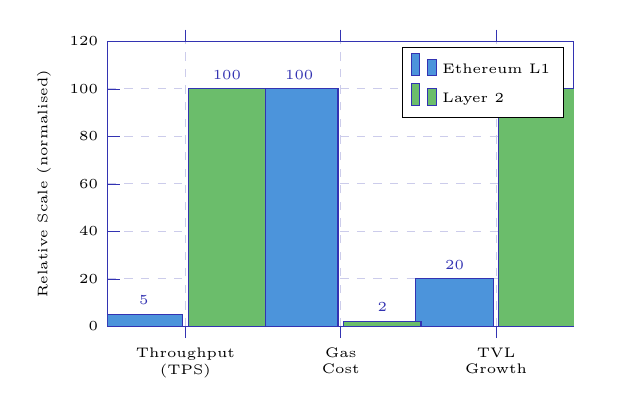
\begin{tikzpicture}
\begin{axis}[
  ybar,
  bar width=28pt,
  width=7.5cm,
  height=5.2cm,
  symbolic x coords={Throughput, Gas Cost, TVL Growth},
  xtick=data,
  xticklabels={Throughput\\(TPS), Gas\\Cost, TVL\\Growth},
  xticklabel style={font=\tiny, text width=2.5cm, align=center},
  ymin=0, ymax=120,
  ytick={0,20,40,60,80,100,120},
  yticklabel style={font=\tiny},
  ylabel style={font=\tiny},
  ylabel={Relative Scale (normalised)},
  axis line style={draw=mlpurple},
  tick style={draw=mlpurple},
  nodes near coords,
  nodes near coords style={font=\tiny, color=mlpurple},
  point meta=y,
  enlarge x limits=0.25,
  grid=major,
  grid style={dashed, mllavender3},
  legend style={font=\tiny, at={(0.98,0.98)}, anchor=north east},
  legend cell align=left,
]
\addplot[fill=mlblue!70,   draw=mlpurple] coordinates {(Throughput, 5)(Gas Cost, 100)(TVL Growth, 20)};
\addplot[fill=mlgreen!70,  draw=mlpurple] coordinates {(Throughput, 100)(Gas Cost, 2)(TVL Growth, 100)};
\legend{Ethereum L1, Layer 2}
\end{axis}
\end{tikzpicture}
\end{column}
\begin{column}{0.36\textwidth}
\vspace{4mm}
\begin{block}{Key Metrics}
\begin{itemize}\setlength\itemsep{4pt}
  \item[\small$\checkmark$] \small \textbf{\$30B+} TVL across L2s
  \item[\small$\checkmark$] \small \textbf{50x} cheaper transactions
  \item[\small$\checkmark$] \small \textbf{100x+} throughput improvement
  \item[\small$\checkmark$] \small \textbf{10+} major L2s live today
\end{itemize}
\end{block}
\end{column}
\end{columns}
\bottomnote{Layer 2 solutions resolve Ethereum's scalability trilemma: higher throughput and lower fees while inheriting L1 security guarantees.}
\end{frame}

% Frame 3: L2 Ecosystem at a Glance
\begin{frame}{L2 Ecosystem at a Glance}
\vspace{2mm}
\begin{center}
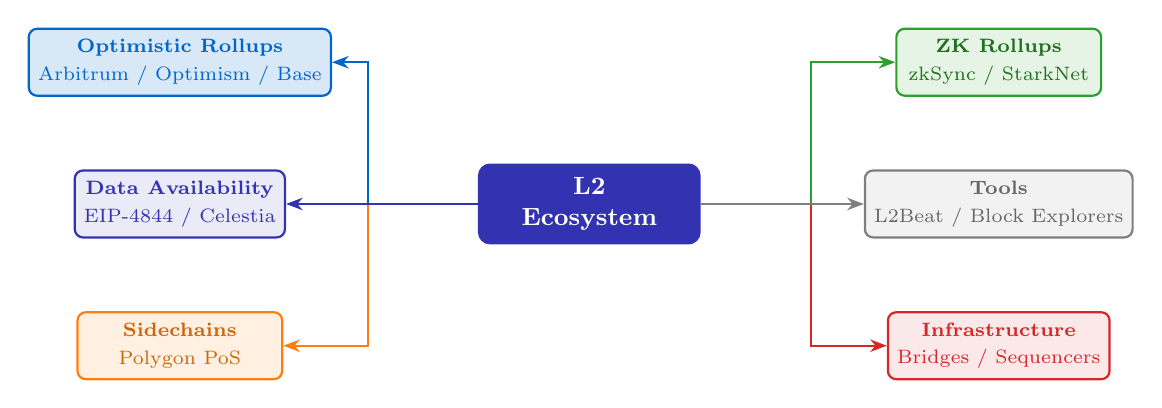
\begin{tikzpicture}[
  cbox/.style={rectangle, rounded corners=4pt, draw=mlpurple, thick,
               fill=mlpurple, minimum width=2.8cm, minimum height=1.0cm,
               font=\small\bfseries, align=center, text=white},
  sbox/.style={rectangle, rounded corners=3pt, thick,
               minimum width=2.6cm, minimum height=0.85cm,
               font=\scriptsize, align=center},
  arr/.style={-{Stealth[length=6pt]}, thick}
]
% Center node
\node[cbox] (center) at (0,0) {L2\\Ecosystem};

% Spoke nodes
\node[sbox, draw=mlblue,   fill=mlblue!15,   text=mlblue]              (opt)   at (-5.2, 1.8)
  {\textbf{Optimistic Rollups}\\[2pt]Arbitrum / Optimism / Base};

\node[sbox, draw=mlgreen,  fill=mlgreen!12,  text=mlgreen!70!black]    (zk)    at ( 5.2, 1.8)
  {\textbf{ZK Rollups}\\[2pt]zkSync / StarkNet};

\node[sbox, draw=mlorange, fill=mlorange!12, text=mlorange!80!black]   (side)  at (-5.2,-1.8)
  {\textbf{Sidechains}\\[2pt]Polygon PoS};

\node[sbox, draw=mlred,    fill=mlred!10,    text=mlred]               (infra) at ( 5.2,-1.8)
  {\textbf{Infrastructure}\\[2pt]Bridges / Sequencers};

\node[sbox, draw=mlpurple, fill=mlpurple!10, text=mlpurple]            (da)    at (-5.2, 0.0)
  {\textbf{Data Availability}\\[2pt]EIP-4844 / Celestia};

\node[sbox, draw=mlgray,   fill=mlgray!10,   text=mlgray!80!black]     (tools) at ( 5.2, 0.0)
  {\textbf{Tools}\\[2pt]L2Beat / Block Explorers};

% Arrows
\draw[arr, draw=mlblue]   (center.west) -- ++(-1.4,0) |- (opt.east);
\draw[arr, draw=mlgreen]  (center.east) -- ++(1.4,0)  |- (zk.west);
\draw[arr, draw=mlorange] (center.west) -- ++(-1.4,0) |- (side.east);
\draw[arr, draw=mlred]    (center.east) -- ++(1.4,0)  |- (infra.west);
\draw[arr, draw=mlpurple] (center.west) -- ++(-1.4,0) |- (da.east);
\draw[arr, draw=mlgray]   (center.east) -- ++(1.4,0)  |- (tools.west);
\end{tikzpicture}
\end{center}
\bottomnote{The L2 ecosystem spans rollup technologies, sidechain solutions, data availability layers, and the infrastructure connecting them to Ethereum.}
\end{frame}

% Frame 4: L2 TVL Growth Trajectory
\begin{frame}{L2 TVL Growth Trajectory}
\begin{columns}[T]
\begin{column}{0.62\textwidth}
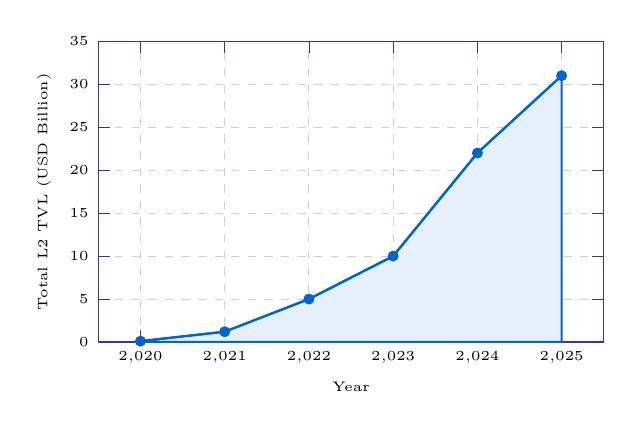
\begin{tikzpicture}
\begin{axis}[
  width=8.0cm,
  height=5.4cm,
  xmin=2019.5, xmax=2025.5,
  ymin=0, ymax=35,
  xtick={2020,2021,2022,2023,2024,2025},
  ytick={0,5,10,15,20,25,30,35},
  xticklabel style={font=\tiny},
  yticklabel style={font=\tiny},
  xlabel style={font=\tiny},
  ylabel style={font=\tiny},
  xlabel={Year},
  ylabel={Total L2 TVL (USD Billion)},
  axis line style={draw=mlpurple},
  tick style={draw=mlpurple},
  grid=major,
  grid style={dashed, mllavender3},
]
\addplot[color=mlblue, solid, thick, mark=*, mark size=1.5pt,
         fill=mlblue!10] coordinates {
  (2020,0.1)(2021,1.2)(2022,5.0)(2023,10.0)(2024,22.0)(2025,31.0)
} \closedcycle;
\addplot[color=mlblue, solid, thick, mark=*, mark size=1.5pt] coordinates {
  (2020,0.1)(2021,1.2)(2022,5.0)(2023,10.0)(2024,22.0)(2025,31.0)
};
\end{axis}
\end{tikzpicture}
\end{column}
\begin{column}{0.36\textwidth}
\vspace{4mm}
\begin{block}{Growth Drivers}
\begin{itemize}\setlength\itemsep{4pt}
  \item[\small$\checkmark$] \small \textbf{DeFi migration} to cheaper L2 rails
  \item[\small$\checkmark$] \small \textbf{EIP-4844} blob fee reduction in 2024
  \item[\small$\checkmark$] \small \textbf{Institutional} adoption of rollup chains
  \item[\small$\checkmark$] \small \textbf{Gaming and NFTs} shifting on-chain activity
\end{itemize}
\end{block}
\end{column}
\end{columns}
\bottomnote{L2 TVL grew from under \$100M in 2020 to over \$30B by 2025, accelerating sharply after EIP-4844 reduced blob fees by up to 90\%.}
\end{frame}

% Frame 5: Course Coverage
\begin{frame}{Course Coverage}
\vspace{2mm}
\begin{center}
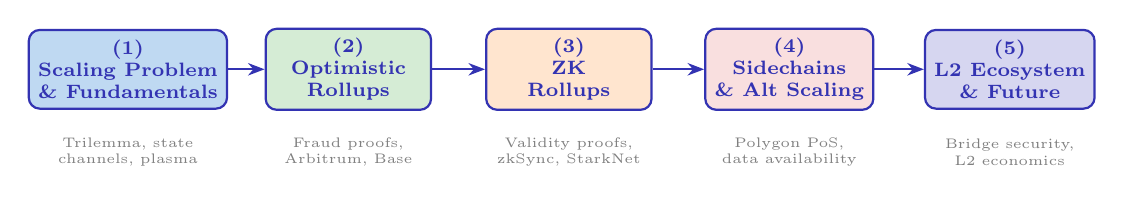
\begin{tikzpicture}[
  procstep/.style={
    rectangle, rounded corners=4pt,
    minimum width=2.1cm, minimum height=1.0cm,
    draw=mlpurple, thick,
    fill=mllavender3,
    font=\scriptsize\bfseries,
    align=center,
    text=mlpurple
  },
  conn/.style={-{Stealth[length=6pt]}, thick, draw=mlpurple}
]
\node[procstep, fill=mlblue!25]    (s1) at (0,0)    {(1)\\Scaling Problem\\\& Fundamentals};
\node[procstep, fill=mlgreen!20]   (s2) at (2.8,0)  {(2)\\Optimistic\\Rollups};
\node[procstep, fill=mlorange!20]  (s3) at (5.6,0)  {(3)\\ZK\\Rollups};
\node[procstep, fill=mlred!15]     (s4) at (8.4,0)  {(4)\\Sidechains\\\& Alt Scaling};
\node[procstep, fill=mlpurple!20]  (s5) at (11.2,0) {(5)\\L2 Ecosystem\\\& Future};

\draw[conn] (s1) -- (s2);
\draw[conn] (s2) -- (s3);
\draw[conn] (s3) -- (s4);
\draw[conn] (s4) -- (s5);

\node[font=\tiny, text=mlgray, align=center, text width=2.1cm] at (0,-1.05)
  {Trilemma, state\\channels, plasma};
\node[font=\tiny, text=mlgray, align=center, text width=2.1cm] at (2.8,-1.05)
  {Fraud proofs,\\Arbitrum, Base};
\node[font=\tiny, text=mlgray, align=center, text width=2.1cm] at (5.6,-1.05)
  {Validity proofs,\\zkSync, StarkNet};
\node[font=\tiny, text=mlgray, align=center, text width=2.1cm] at (8.4,-1.05)
  {Polygon PoS,\\data availability};
\node[font=\tiny, text=mlgray, align=center, text width=2.1cm] at (11.2,-1.05)
  {Bridge security,\\L2 economics};
\end{tikzpicture}
\end{center}
\vspace{4mm}
\begin{columns}[T]
\begin{column}{0.48\textwidth}
\begin{block}{Prerequisites}
\begin{itemize}\setlength\itemsep{2pt}
  \item[\small$\checkmark$] \small Basic blockchain and Ethereum knowledge
  \item[\small$\checkmark$] \small Introductory smart contract concepts
\end{itemize}
\end{block}
\end{column}
\begin{column}{0.48\textwidth}
\begin{block}{Outcomes}
\begin{itemize}\setlength\itemsep{2pt}
  \item[\small$\checkmark$] \small Evaluate rollup designs and trade-offs
  \item[\small$\checkmark$] \small Assess bridge security and L2 economics
\end{itemize}
\end{block}
\end{column}
\end{columns}
\bottomnote{Five modules progress from foundational scaling theory to hands-on analysis of live rollup ecosystems and their economic models.}
\end{frame}

% Frame 6: What You Will Learn
\begin{frame}{What You Will Learn}
\begin{columns}[T]
\begin{column}{0.44\textwidth}
\vspace{2mm}
\begin{block}{Learning Outcomes}
\begin{itemize}\setlength\itemsep{5pt}
  \item[\small$\checkmark$] \small \textbf{L2 architecture} --- rollup design, sequencers, settlement layers
  \item[\small$\checkmark$] \small \textbf{Rollup mechanics} --- fraud proofs, validity proofs, challenge windows
  \item[\small$\checkmark$] \small \textbf{Proof systems} --- ZK-SNARKs, ZK-STARKs, recursive proving
  \item[\small$\checkmark$] \small \textbf{Bridge security} --- cross-chain messaging risks, exit mechanisms
  \item[\small$\checkmark$] \small \textbf{L2 economics} --- fee models, sequencer incentives, MEV on L2
\end{itemize}
\end{block}
\end{column}
\begin{column}{0.54\textwidth}
\vspace{2mm}
\begin{center}
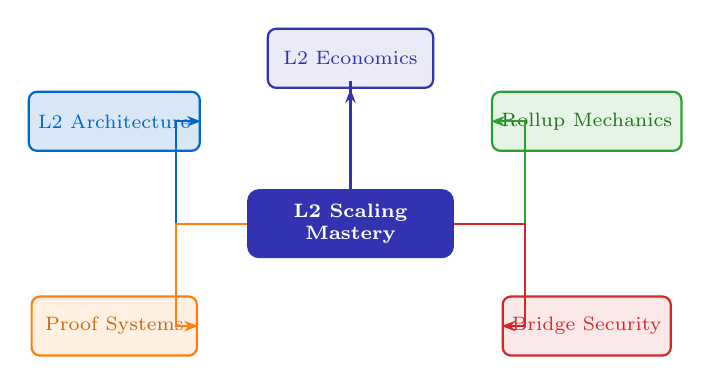
\begin{tikzpicture}[
  cbox/.style={rectangle, rounded corners=4pt, draw=mlpurple, thick,
               fill=mlpurple, minimum width=2.6cm, minimum height=0.85cm,
               font=\scriptsize\bfseries, align=center, text=white},
  fbox/.style={rectangle, rounded corners=3pt, thick,
               minimum width=2.1cm, minimum height=0.75cm,
               font=\scriptsize, align=center},
  farr/.style={-{Stealth[length=5pt]}, thick}
]
% Central node
\node[cbox] (nm) at (0,0) {L2 Scaling\\Mastery};

% Skill nodes
\node[fbox, draw=mlblue,   fill=mlblue!15,   text=mlblue]              (arch) at (-3.0, 1.3) {L2 Architecture};
\node[fbox, draw=mlgreen,  fill=mlgreen!12,  text=mlgreen!70!black]    (roll) at ( 3.0, 1.3) {Rollup Mechanics};
\node[fbox, draw=mlorange, fill=mlorange!12, text=mlorange!80!black]   (prf)  at (-3.0,-1.3) {Proof Systems};
\node[fbox, draw=mlred,    fill=mlred!10,    text=mlred]               (bri)  at ( 3.0,-1.3) {Bridge Security};
\node[fbox, draw=mlpurple, fill=mlpurple!10, text=mlpurple]            (eco)  at ( 0.0, 2.1) {L2 Economics};

% Arrows
\draw[farr, draw=mlblue]   (nm.west)  -- ++(-0.9,0) |- (arch.east);
\draw[farr, draw=mlgreen]  (nm.east)  -- ++(0.9,0)  |- (roll.west);
\draw[farr, draw=mlorange] (nm.west)  -- ++(-0.9,0) |- (prf.east);
\draw[farr, draw=mlred]    (nm.east)  -- ++(0.9,0)  |- (bri.west);
\draw[farr, draw=mlpurple] (nm.north) -- ++(0,0.6)  |- (eco.south);
\end{tikzpicture}
\end{center}
\end{column}
\end{columns}
\vspace{1mm}
\bottomnote{By the end you will be able to design, compare, and audit Layer 2 solutions with deep knowledge of rollup proofs, bridges, and economic models.}
\end{frame}

\end{document}
